% Generated by `python -m experiments.experiment_4.appendix_captions` -- do not edit by hand.
% DRAFT: ?? marks values whose source file was absent. Do not commit.
% Main-text figure for Experiment 4. Needs \usepackage{graphicx}; paths are relative to outputs/finals/experiment-4/.
\begin{figure}[tbp]
  \centering
  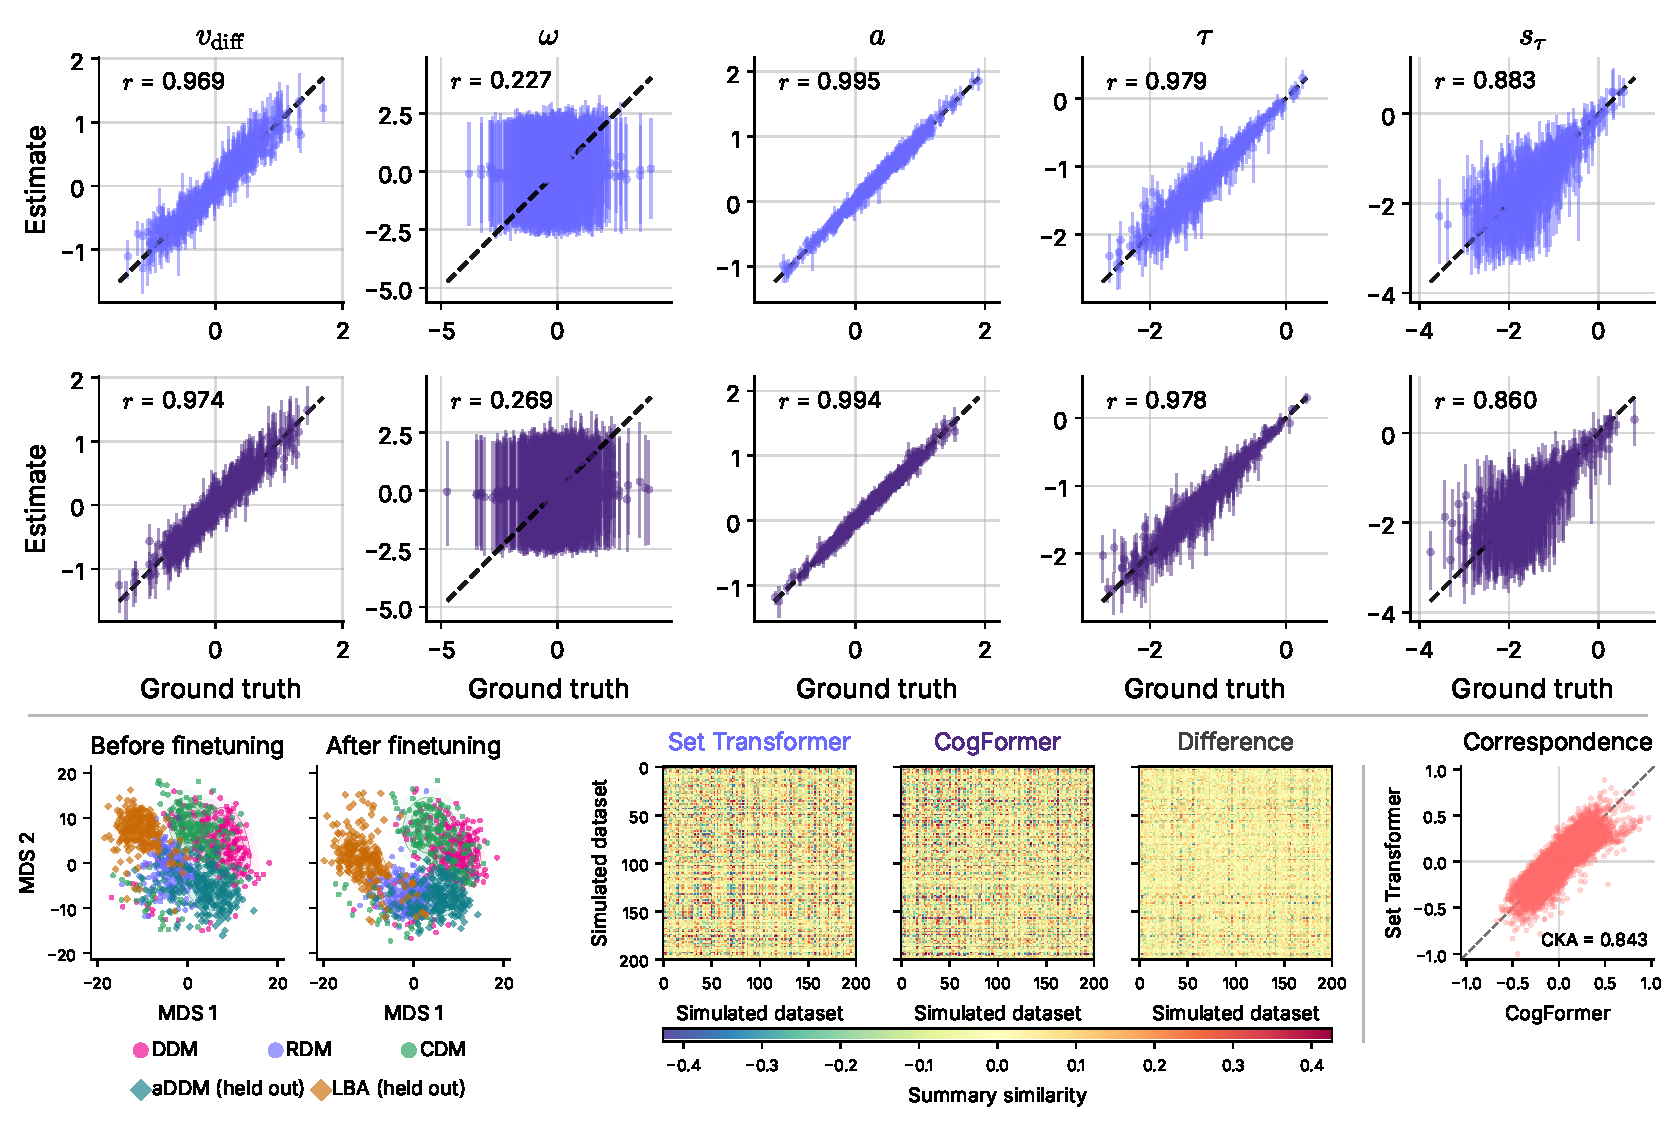
\includegraphics[width=\textwidth]{probe/compare/panel.pdf}
  \caption{\textbf{A frozen CogFormer encoder as the summary network for a held-out model.} \emph{Top:} parameter recovery for the attentional DDM (aDDM; five free parameters), a family the encoder never saw, by two amortized posteriors that share the same FlowMatching network and training budget and differ only in the summary: a SetTransformer learned for this task (upper row, light) and CogFormer's frozen encoder (lower row, dark). Points are posterior medians against ground truth with 95\% credible intervals, on the unconstrained scale, for \textbf{??} validation datasets per arm; $r$ is their correlation. $\omega$ is barely identified in this design (posterior contraction 0.07 and 0.06 in the two arms). \emph{Bottom left:} two-dimensional MDS of the frozen encoder's summaries of \textbf{??} datasets per family, for the three training families (circles) and the two held-out ones (diamonds), before and after fine-tuning on the LBA (Experiment~3); one joint fit, so both panels share axes, with per-family density contours. \emph{Bottom right:} how the two summaries organise the same \textbf{??} aDDM datasets: normalised Gram matrices (pairwise similarity between datasets) of the learned and the frozen summary, their difference, and their off-diagonal entries against each other, with linear CKA. Details in Appendix~\ref{app:exp4-main-details}.}
  \label{fig:exp4-main}
\end{figure}
